\ffigbox[\FBwidth]{%
\caption{\centering Graphe \(G\) avec un 4-cycle \(C\) et deux 2-sommets voisins \(x\) et \(y\)}\label{fig:c4_plus_2_plus_2}
}{
    \fbox{
        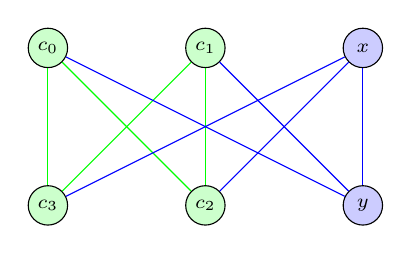
\begin{tikzpicture}[scale=1, main node/.style={circle, draw, fill=blue!20, inner sep=1pt, font=\scriptsize, minimum size=5mm, text=black}]
            
            % construction de C
            \node[main node, fill=green!20] (c0) at (0,2) {\(c_0\)};
            \node[main node, fill=green!20] (c1) at (2,2) {\(c_1\)};
            \node[main node, fill=green!20] (c2) at (2,0) {\(c_2\)};
            \node[main node, fill=green!20] (c3) at (0,0) {\(c_3\)};

            \draw[draw=green] (c0) -- (c2);
            \draw[draw=green] (c1) -- (c2);
            \draw[draw=green] (c1) -- (c3);
            \draw[draw=green] (c3) -- (c0);

            % rajout du 2-sommet
            \node[main node, fill=blue!20] (x) at (4, 2) {\(x\)};
            \node[main node, fill=blue!20] (y) at (4, 0) {\(y\)};
            
            \draw[draw=blue] (x) -- (c2);
            \draw[draw=blue] (x) -- (c3);
            \draw[draw=blue] (y) -- (c0);
            \draw[draw=blue] (y) -- (c1);
            \draw[draw=blue] (x) -- (y);
        \end{tikzpicture}
    }
}